%!TEX root = ./proposta.tex

A Cloud architecture involves communication among countless components through the Web Service's Application Programming Interface (API). The users of this architecture don't know and do not need to know about the localization of their data or applications they wish to use, but they depend on the present security level, which is a concern topic for administrators. Security in Clouds concern data security and network security, according to \cite{Dhage:2011:IDS:1980022.1980076}. 

While an attack against data affects a restrict number of users, an attack against the network compromises many users at the same time. DDoS attacks against a Cloud are attacks against the network availability, and are of critical matter.

Due to the new infrastructure of resources created by the Clouds, there is the possibility of moving physically an application to another address, while it is under a DDoS attack. Therefore, fault-tolerance and resources conservation can be obtained, since this new address will only be known by authentic clients.

This work proposes an architecture to mitigate DDoS attacks in Clouds in a autonomous and independent way. The differences between this proposal to other are majorly in the independence of the hosted application, in providing accuracy in the filter for authentic traffic, for not financially burden the resources use and for minimize the problems caused by the attack without human intervention. The proposed architecture could be used by any web application hosted on a Cloud, that, when notice evidence of a DDoS attack, will filter the authentic traffic and redirects only those to a new instance of the same application.


\begin{figure}[h!]
\centering
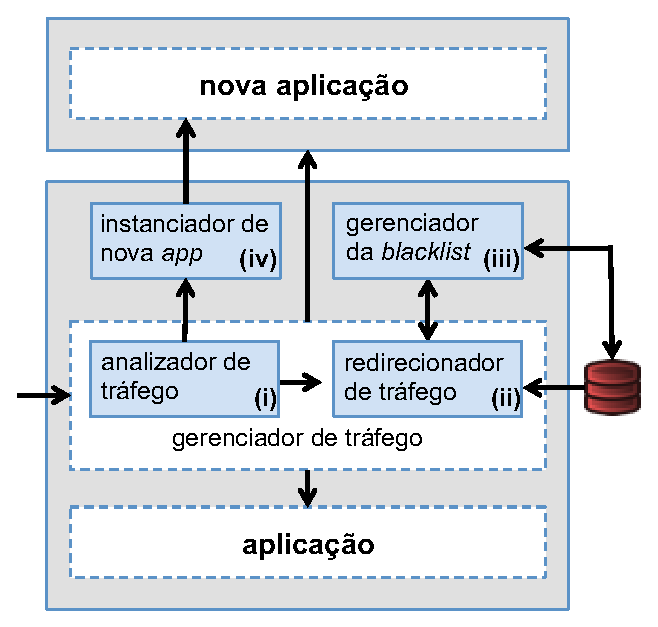
\includegraphics[width=0.55\textwidth]{images/arq.eps}
\caption{Illustration of the proposed architecture for mitigating DDoS attacks}
\label{fig:arq}
\end{figure}

This architecture, illustrated in the figure \ref{fig:arq}, is composed by a general module called Traffic Manager (TM), that does not communicates directly to the application. It is worth noticing that the database instance must be outside any other instance in the Cloud, due to the fact that this database, which is also in the Cloud, may be reached from any other application instance in the Cloud. The operations performed by the TM module are divided in four submodules.

The Traffic Analyzer (TA) submodule watches the behavior of the incoming traffic proactively. Focusing on the approximation of the traffic amount and CPU use on the host, this submodule performs probes to identify the existence of a DDoS attack. In case it is detected, the New Application Instantiator (NAI) module is activated. The NAI will create a new instance of the application in another server in the Cloud, which will consequently have a different IP address\footnote{When the instance is created, the old one will be deactivated. The first instance in the Cloud will only redirect traffic}. Thus, the Traffic Redirector (TR) submodule will receive and process all the incoming traffic, responding with a redirect to the new instance of the application. We're assuming that DDoS attacks do not interpret any responses from the server, since its effectiveness would be diminished if it did. This way, only authentic clients will be redirected to the new application.

When a client is redirected to the new instance, this client's address, whether it is authentic or not, will be inserted into a blacklist. The clients in this blacklist will have their requests ignored, intending to reduce the overhead in the server. Nonetheless, since the legitimate client was informed of the new application before its address was inserted in this list, that will not be a problem, for it will have access to the new application. All the entries in the blacklist will have a limited time to live (TTL), since a response can be lost. The TTL for each entry will increase exponentially, in order to reduce even more the overload. It is the Blacklist Manager (BM) duty to take an address out of the blacklist, and also to calculate the exponentially growing TTL.

However, in order to prevent that this control stops the access of the legitimate clients in their future requests, the client, when redirected, shall have this new address stored as a cookie in their computer. This procedure makes sure only authentic clients have knowledge of the new address of the application, and thus the traffic redirection may be recursively repeated, until a maximum predetermined level.

The figure~\ref{fig:cen} illustrates a scenario under DDoS attack, where the clients are represented by icons of many internet browsers, and the spaceship is the icon of the application called LOIC -- Low Orbit Ion Cannon. To the left, all of them send their traffic to what they imagine is the instance of the application. Considering a situation where the application is under attack, it will be replicated, and the original instance will redirect the legitimate traffic to the new application. To the right, the redirection result is shown: genuineclients can reach the new instance of the application, while the attackers keep attacking the old instance, that now operates only redirecting traffic.


\begin{figure}[t!]
	\centering
	\includegraphics[width=0.40\textwidth]{images/an1.eps}
	% \caption{bla}
	\hskip 1cm
	\includegraphics[width=0.40\textwidth]{images/an2.eps}
	\caption{traffic behavior under an attack scenario}
	\label{fig:cen}
\end{figure}
